\documentclass[tikz, border=10pt]{standalone}
\usepackage{amsmath, amssymb, xcolor}
% Load the necessary libraries correctly
\usetikzlibrary{matrix, fit, backgrounds, positioning, calc}

\begin{document}
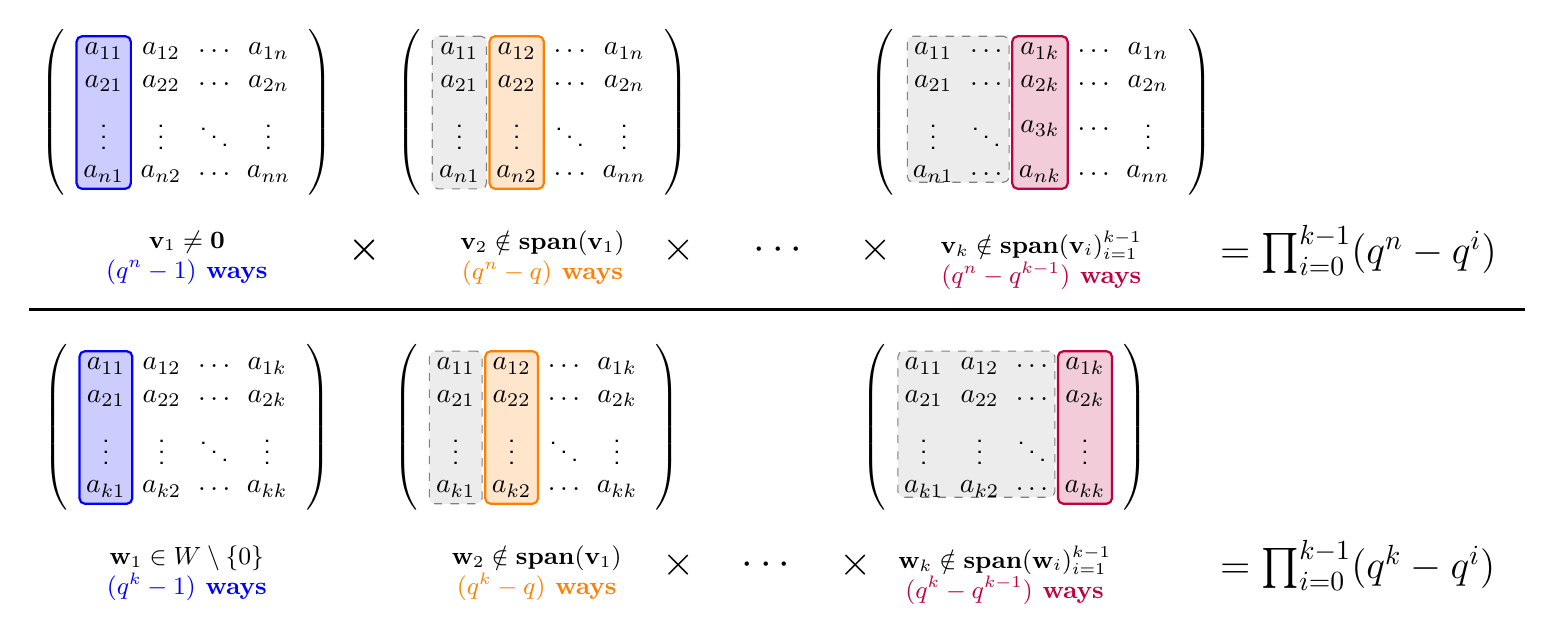
\begin{tikzpicture}[
	font=\sffamily,
	% Corrected Matrix Style
	mtx/.style={
		matrix of math nodes,
		left delimiter=(, right delimiter=),
		nodes={minimum width=1.2em, inner sep=2pt, anchor=center},
		column sep=2pt, row sep=2pt,
		ampersand replacement=\&
	},
	% Highlighting styles
	hl-v1/.style={fill=blue!20, draw=blue, thick, rounded corners=2pt, inner sep=.25pt},
	hl-v2/.style={fill=orange!20, draw=orange, thick, rounded corners=2pt, inner sep=.25pt},
	hl-vi/.style={fill=purple!20, draw=purple, thick, rounded corners=2pt, inner sep=.25pt},
	hl-span/.style={fill=gray!15, draw=gray, dashed, rounded corners=2pt, inner sep=.25pt},
	% Text styles
	mainTitle/.style={font=\sffamily\bfseries\LARGE, color=darkgray},
	term label/.style={font=\bfseries\small, align=center},
	box/.style={draw=black!30, fill=white, rounded corners=5pt, inner sep=15pt}
	]
	
	% ==============================================================================
	% PATH 1: COUNTING DIRECTLY IN F_q^n
	% ==============================================================================
%	\node[mainTitle, anchor=west] at (-1, 4) {1. Direct Count of $\Omega$ in $\mathbb{F}_q^n$};
	
	\begin{scope}[shift={(0, 0)}]
		% v1 selection
		\matrix[mtx] (N1) { 
			a_{11} \& a_{12} \& \dots \& a_{1n} \\ 
			a_{21} \& a_{22} \& \dots \& a_{2n} \\ 
			\vdots \& \vdots \& \ddots \& \vdots \\ 
			a_{n1} \& a_{n2} \& \dots \& a_{nn} \\ 
		};
		\begin{scope}[on background layer] 
			\node[hl-v1, fit=(N1-1-1)(N1-4-1)] {}; 
		\end{scope}
		\node[below=0.3cm of N1, term label] {$\textbf{v}_1 \neq \textbf{0}$ \\ \textcolor{blue}{$(q^n - 1)$ ways}};
		
		% v2 selection
		\matrix[mtx, right=1.5cm of N1] (N2) { 
			a_{11} \& a_{12} \& \dots \& a_{1n} \\ 
			a_{21} \& a_{22} \& \dots \& a_{2n} \\ 
			\vdots \& \vdots \& \ddots \& \vdots \\ 
			a_{n1} \& a_{n2} \& \dots \& a_{nn} \\ 
		};
		\begin{scope}[on background layer] 
			\node[hl-span, fit=(N2-1-1)(N2-4-1)] {}; 
			\node[hl-v2, fit=(N2-1-2)(N2-4-2)] {}; 
		\end{scope}
		\node[below=0.3cm of N2, term label] {$\textbf{v}_2 \notin \text{span}(\textbf{v}_1)$ \\ \textcolor{orange}{$(q^n - q)$ ways}};
		
		% vk selection
		\matrix[mtx, right=3cm of N2] (Nk) { 
			a_{11} \& \dots  \& a_{1k} \& \dots  \& a_{1n} \\ 
			a_{21} \& \dots  \& a_{2k} \& \dots  \& a_{2n} \\ 
			\vdots \& \ddots \& a_{3k} \& \dots  \& \vdots \\ 
			a_{n1} \& \dots  \& a_{nk} \& \dots  \& a_{nn} \\ 
		};
		\begin{scope}[on background layer] 
			\node[hl-span, fit=(Nk-1-1)(Nk-4-2)] {}; 
			\node[hl-vi, fit=(Nk-1-3)(Nk-4-3)] {}; 
		\end{scope}
		\node[below=0.3cm of Nk, term label] {$\textbf{v}_k \notin \text{span}(\textbf{v}_i)_{i=1}^{k-1}$ \\ \textcolor{purple}{$(q^n - q^{k-1})$ ways}};
		
		\node[scale=1.5] at ($(N1)!0.5!(N2)+(0,-1.75)$) {$\times$};
		\node[scale=1.5] at (6.25,-1.75) {$\times$};
		\node[scale=1.5] at (7.55,-1.75) {$\cdots$};
		\node[scale=1.5] at (8.75,-1.75) {$\times$};
		
		\node[anchor=west, font=\bfseries\Large] (Total1) at (13, -1.75) {$= \prod_{i=0}^{k-1} (q^n - q^i)$};
	\end{scope}
	
	\draw[very thick] (-2, -2.5) -- (17, -2.5);
	
	% ==============================================================================
	% PATH 2: COUNTING VIA SUBSPACE W
	% ==============================================================================
	
	\begin{scope}[shift={(0, -4)}]
%		% The number of subspaces
%		\node[draw=orange, fill=orange!5, inner sep=10pt, font=\bfseries\large, rounded corners=3pt] (Nsub) at (-0.5, 0) {Subspaces $W$ \\ (Count = $N$)};
%		\node[scale=2] at (1.5, 0) {$\times$};
		
		% Bases inside W (W is k-dimensional)
		\matrix[mtx] (W1) { 
			a_{11} \& a_{12} \& \dots \& a_{1k} \\ 
			a_{21} \& a_{22} \& \dots \& a_{2k} \\ 
			\vdots \& \vdots \& \ddots \& \vdots \\ 
			a_{k1} \& a_{k2} \& \dots \& a_{kk} \\ 
		};
		\begin{scope}[on background layer] 
			\node[hl-v1, fit=(W1-1-1)(W1-4-1)] {}; 
		\end{scope}
		\node[below=0.3cm of W1, term label] {$\textbf{w}_1 \in W \setminus \{0\}$ \\ \textcolor{blue}{$(q^k - 1)$ ways}};
		
		\matrix[mtx, right=1.5cm of W1] (W2) { 
			a_{11} \& a_{12} \& \dots \& a_{1k} \\ 
			a_{21} \& a_{22} \& \dots \& a_{2k} \\ 
			\vdots \& \vdots \& \ddots \& \vdots \\ 
			a_{k1} \& a_{k2} \& \dots \& a_{kk} \\ 
		};
		\begin{scope}[on background layer] 
			\node[hl-span, fit=(W2-1-1)(W2-4-1)] {}; 
			\node[hl-v2, fit=(W2-1-2)(W2-4-2)] {}; 
		\end{scope}
		\node[below=0.3cm of W2, term label] {$\textbf{w}_2 \notin \text{span}(\textbf{v}_1)$ \\ \textcolor{orange}{$(q^k - q)$ ways}};
		
		
		\matrix[mtx, right=3cm of W2] (Wk) { 
			a_{11} \& a_{12} \& \dots \& a_{1k} \\ 
			a_{21} \& a_{22} \& \dots \& a_{2k} \\ 
			\vdots \& \vdots \& \ddots \& \vdots \\ 
			a_{k1} \& a_{k2} \& \dots \& a_{kk} \\ 
		};
		\begin{scope}[on background layer] 
			\node[hl-span, fit=(Wk-1-1)(Wk-4-3)] {}; 
			\node[hl-vi, fit=(Wk-1-4)(Wk-4-4)] {}; 
		\end{scope}
		\node[below=0.3cm of Wk, term label] {$\textbf{w}_k \notin \text{span}(\textbf{w}_i)_{i=1}^{k-1}$ \\ \textcolor{purple}{$(q^k - q^{k-1})$ ways}};
%		
%		\node at ($(W1)!0.5!(Wk)$) {\dots};
%		\node[anchor=west, font=\bfseries\Large] (Total2) at (10, 0) {$= N \cdot \prod_{i=0}^{k-1} (q^k - q^i)$};
		\node[scale=1.5] at ($(N1)!0.5!(N2)+(0,-1.75)$) {$\times$};
		\node[scale=1.5] at (6.25,-1.75) {$\times$};
		\node[scale=1.5] at (7.4,-1.75) {$\cdots$};
		\node[scale=1.5] at (8.5,-1.75) {$\times$};
		
		\node[anchor=west, font=\bfseries\Large] (Total1) at (13, -1.75) {$= \prod_{i=0}^{k-1} (q^k - q^i)$};
	\end{scope}
	
%	% ==============================================================================
%	% FINAL EQUIVALENCE
%	% ==============================================================================
%	\node[box, below=2cm of Total2, xshift=-4cm] (Final) {
%		\large \textbf{Equating Paths:} \\[8pt]
%		$\displaystyle N \cdot \prod_{i=0}^{k-1} (q^k - q^i) = \prod_{i=0}^{k-1} (q^n - q^i) $ \\[15pt]
%		$\displaystyle N = \frac{(q^n-1)(q^n-q)\cdots(q^n-q^{k-1})}{(q^k-1)(q^k-q)\cdots(q^k-q^{k-1})} = \binom{n}{k}_q$
%	};
	
\end{tikzpicture}
\end{document}